\documentclass{beamer}
\usepackage{graphicx}
\usepackage{paralist}
\usepackage{outlines}

\title{Liquify Filter}
\author{Mendocino College - Digital Image Manipulation with Photoshop}
\titlegraphic{\vspace{-10mm}
\includegraphics[width = .9\textwidth]{images/photoshop.jpg}} 
\date{\vspace{-5em}} 


\mode <presentation>
\usetheme{Warsaw}
\usecolortheme{default}

\setbeamerfont{footline}{size=\fontsize{5}{8}\selectfont}

\definecolor{darkred}{rgb}{20,0,0}
\definecolor{darkgreen}{RGB}{40,110,20}
\definecolor{darkpurple}{RGB}{30,0,30}
\definecolor{chardonnay}{RGB}{255, 255, 204}

\setbeamercolor*{palette primary}{fg=white, bg=darkgreen}


\begin{document}
	{
		\setbeamertemplate{footline}{} 
		\setbeamertemplate{headline}{} 
		\begin{frame}
			\vspace{-35pt}
			\maketitle
		\end{frame}
	}
		
		
\section{Liquify Filter}

\subsection{What is the Liquify Filter?}		

	\begin{frame}
		\frametitle{What is the Liquify Filter?}
		\begin{outline}
			\1 The Liquify filter lets you push, pull, rotate, reflect, pucker, and bloat any area of an image. 
			\1 This allows us to easily manipulate peoples facial features, such as adjusting nose size, or turning a frown into a smile.
			\1 The distortions you create can be subtle or drastic, which makes the Liquify command a powerful tool for retouching images as well as creating artistic effects. 
			\1 Use the filter for subtle retouching tasks, and reach for it to smooth out wrinkles in clothing or rough edges. 
			\1 The Liquify filter is also used to tweak subtle elements, such as facial features.
		\end{outline}
	\end{frame}

\subsection{How to use the Liquify FIlter}		

	\begin{frame}
		\frametitle{How to Apply Liquify as a smart filter}
		\begin{outline}
			\1 First duplicate your image.
			\2 Right click on the layer
			\2 Select:  Duplicate Layer...
			\2 Click:  OK
			\1 Then convert the new layer to a smart object
			\2 Right click on the new layer
			\2 Select:  Convert to Smart Object
			\2 
\includegraphics[width=0.05\textwidth]{images/smart object.png} The layer will have this image over it, when it is a smart object.
		\end{outline}
	\begin{center}
		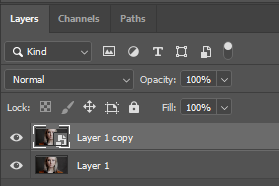
\includegraphics[width=0.35\textwidth]{images/convert to smart object.png}
	\end{center}
	\end{frame}

	\begin{frame}
	\frametitle{How to open the Liquify Filter}
	\begin{outline}
		\1 In the top menu bar, click: Filter
		\2 Select:  Liquify...
		\1 Or hold down the following keys at the same time:
		\2 Shift + Ctrl + X
	\end{outline}
	\begin{center}
	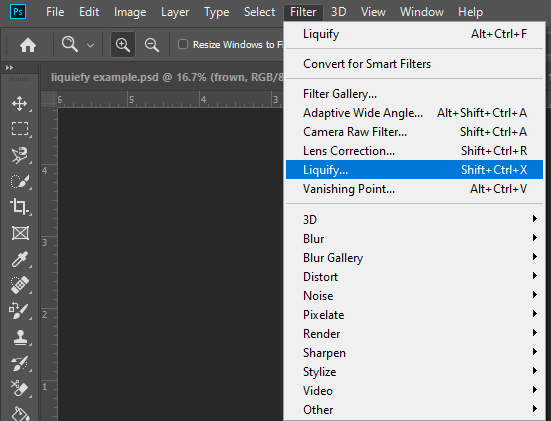
\includegraphics[width=0.75\textwidth]{images/filter - liquify.png}
\end{center}
\end{frame}

	\begin{frame}
	\frametitle{How to use the Liquify Filter}
	\begin{outline}
		\1 This is the Liquify Dialog Box
		\1 The left side contain manual tools for manipulating images.
		\1 The right side contains Panels for various tasks
		\2 The most important Panel for us will be the Brush Tool Options and the Face-Aware Liquify
	\end{outline}
	\begin{center}
	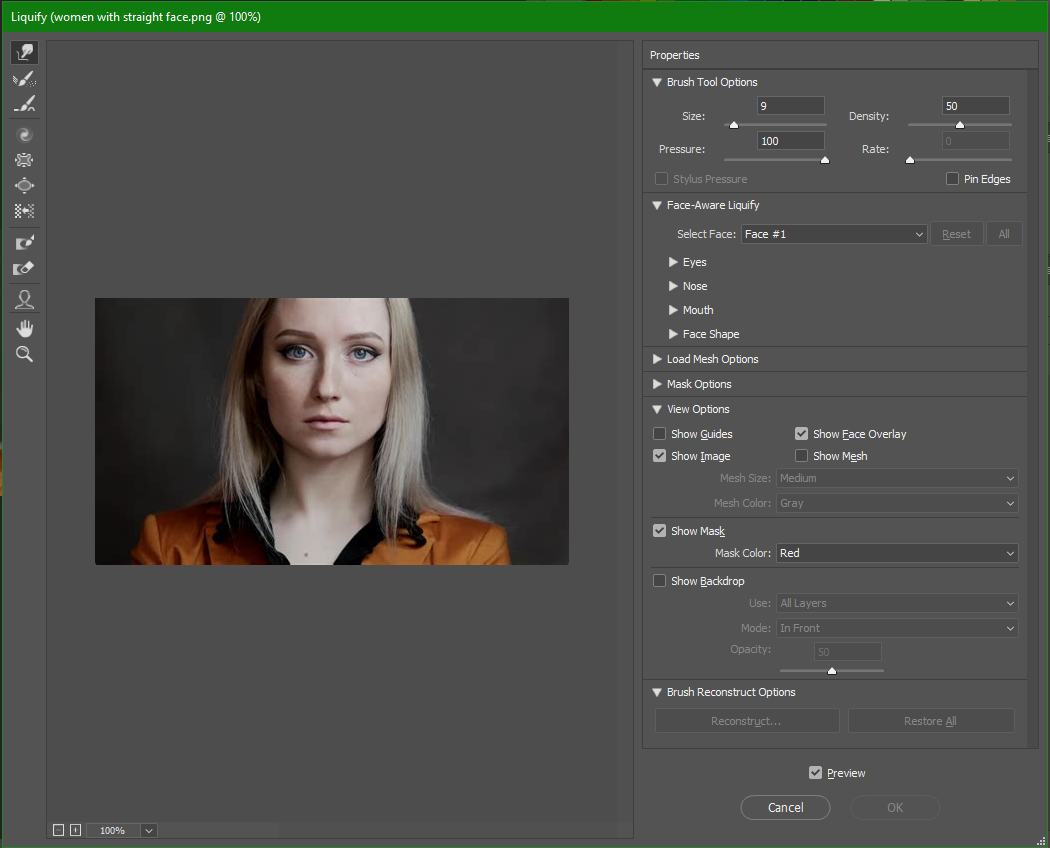
\includegraphics[width=0.65\textwidth]{images/liquify dialog box.png}
\end{center}
\end{frame}


\section{Examples}

\subsection{Bloat Tool}		
\begin{frame}
	\frametitle{Bloat Tool Example}
	\begin{center}
	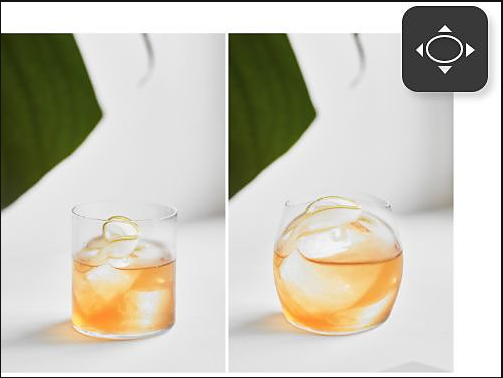
\includegraphics[width=0.65\textwidth]{images/liquify - bloat.png}
\end{center}
\end{frame}

\subsection{Pucker Tool}		
\begin{frame}
	\frametitle{Pucker Tool Example}
	\begin{center}
		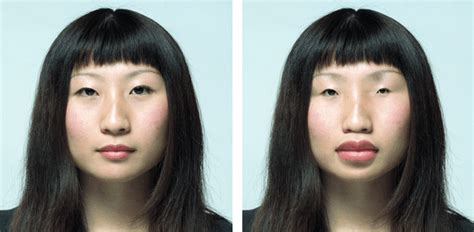
\includegraphics[width=0.65\textwidth]{images/liquify - pucker.jpg}
	\end{center}
\end{frame}

\subsection{Face-Aware Liquify}		
\begin{frame}
	\frametitle{Change face shape and expressions}
	\begin{center}
		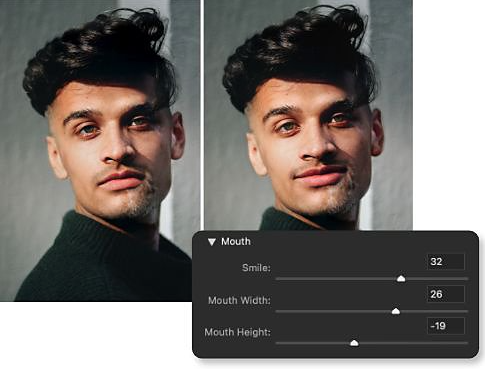
\includegraphics[width=0.65\textwidth]{images/liquify - face.png}
	\end{center}
\end{frame}


\section{Options}

\subsection{Face-Aware Liquify}		

\begin{frame}
	\frametitle{Face-Aware Liquify}
	\begin{outline}
		\1 Allows you to select individual faces and automatically adjust their features. 
	\end{outline}
	\begin{center}
	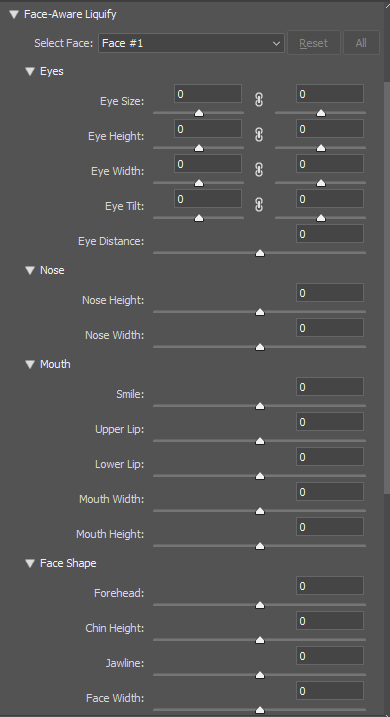
\includegraphics[width=0.35\textwidth]{images/face-aware liquify.png}
\end{center}
\end{frame}

\begin{frame}
	\frametitle{Face Tool}
	\begin{outline}
		\1 Allows you to make the adjustments in the face-aware liquify panel on the fly, with your mouse.
	\end{outline}
	\begin{center}
		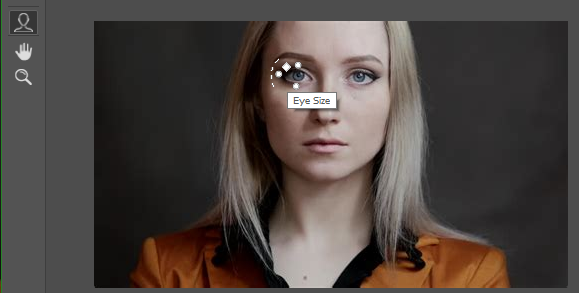
\includegraphics[width=1.0\textwidth]{images/liquify - face tool.png}
	\end{center}
\end{frame}

\subsection{Distortion Tools}		

\begin{frame}
	\frametitle{Distortion Tools}
	\begin{outline}
		\1 The Liquify menu includes several distortion tools that push and pull pixels as if they were water. 
		\2 While Liquify is technically a filter, you can use it as if it were a brush to make changes. 
		\2 Each of these tools has fully customizable tool options to control factors like brush size or brush density.
		\1 Forward Warp tool - 
		\2 Push pixels out of the way as you drag this tool, like running a finger through a pool of liquid.
		\1 Bloat tool - 
		\2 Move pixels away from the center of the brush area, like a bubble emerging from water. 
		\2 Hold down the mouse button to intensify the effect.
		\1 Pucker tool - 
		\2 Push pixels toward the center of the brush area, like water getting sucked into a drain. 
		\2 Hold down the mouse button to intensify the effect.
	\end{outline}
\end{frame}

\begin{frame}
	\frametitle{Distortion Tools}
	\begin{outline}
		\1 Twirl Clockwise tool - 
		\2 Create swirls and eddies of pixels, like tiny whirlpools or forkfuls of spaghetti. 
		\2 Twirls are clockwise by default, with counterclockwise an alternative option.
		\1 Push Left tool - 
		\2 Push pixels left (or right, if you’re using the alternative option) like a miniature bulldozer moving piles of earth.
		\1 Reconstruct tool - 
		\2 This tool reverses distortions you’ve added, calming the waters and restoring the original image beneath your changes.
	\end{outline}
\end{frame}


\subsection{}		
\begin{frame}
	\frametitle{Additional Resources for the Liquify Filter}
	\begin{outline}
		\1 Use the Liquify filter
		\2 By:  Adobe
		\2 https://helpx.adobe.com/photoshop/using/liquify-filter.html
		\1 How to Use the Liquify Tool in Photoshop | Day 12
		\2 PHLEARN
		\2 https://youtu.be/9DLumkDFngk
	\end{outline}
\end{frame}
	
\end{document}